\documentclass{article}
\usepackage[left=1in,top=2in,bottom=1in,right=1in]{geometry}
\usepackage{listings}
\usepackage{graphicx}
\usepackage{hyperref}
\usepackage{breakurl}
\usepackage{subfigure}

\newcommand{\theurl}{\texttt{video.cs.cmu.edu}}

\title{	15-441: Computer Networks\\
Project 3: Video CDN\\
}
\author{\textbf{Lead TAs:}\\ 
             Matt Mukerjee
             $<$\href{mailto:mukerjee@cs.cmu.edu}{mukerjee@cs.cmu.edu}$>$\\
			 David Naylor
             $<$\href{mailto:dnaylor@cs.cmu.edu}{dnaylor@cs.cmu.edu}$>$}
\date{}
\begin{document}
\maketitle

\large{\noindent \textbf{Assigned: 11/7/13\\
Checkpoint 1 due: 11/21/13 (11:59 PM)\\
Final version due: 12/5/13 (11:59 PM)}}


\section{Overview}

In this project you will explore how video content distribution networks (CDNs)
work. In particular, you will implement adaptive bitrate selection, DNS load
balancing, and pieces of OSPF (which your DNS server will use to decide which
server is closest to a given client).

\subsection{In the Real World}

Figure~\ref{fig:overview-real} depicts (at a high level) what this system looks
like in the real world. Clients trying to stream a video first issue a DNS
query to resolve the service's domain name to an IP address for one of the
CDN's content servers. The CDN's authoritative DNS server selects the ``best''
content server for each particular client based on (1) the client's IP address
(from which it learns the client's geographic location) and (2) current load on
the content servers (which the servers periodically report to the DNS server).

Once the client has the IP address for one of the content servers, it begins
requesting chunks of the video the user requested. The video is encoded at
multiple bitrates; as the client player receives video data, it calculates the
throughput of the transfer and requests the highest bitrate the connection can
support.

\begin{figure}
	\centering
	\begin{minipage}{0.4\textwidth}
		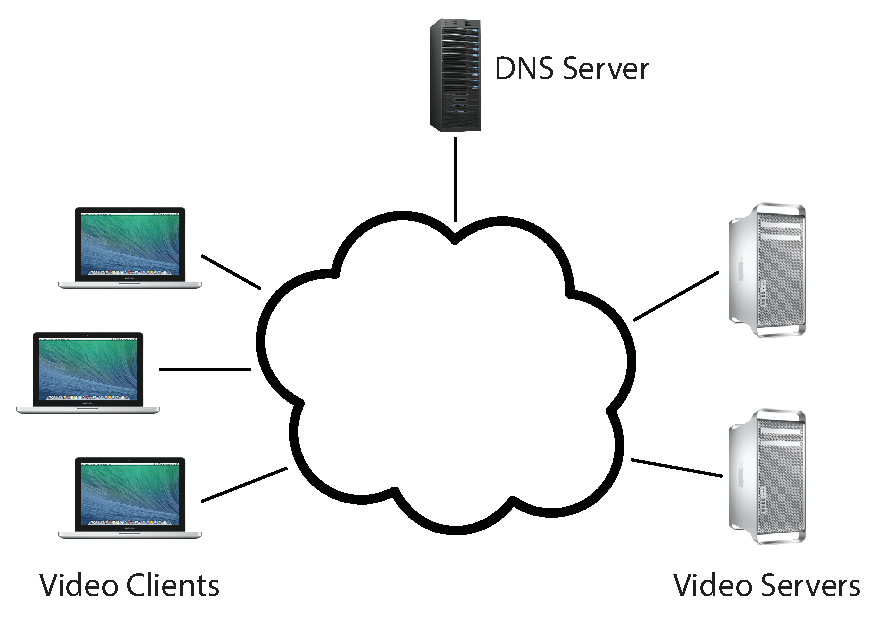
\includegraphics[width=\columnwidth]{figs/overview-real.eps}
		\caption{In the real world...}
		\label{fig:overview-real}
	\end{minipage}
	\hfill
	\begin{minipage}{0.4\textwidth}
		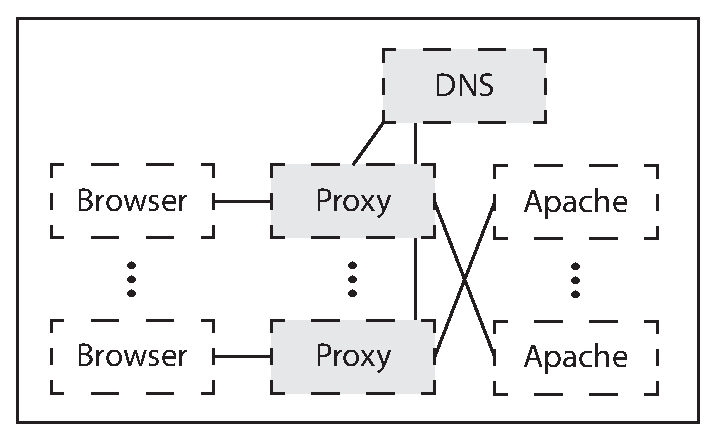
\includegraphics[width=\columnwidth]{figs/overview-fake.eps}
		\caption{Your system.}
		\label{fig:overview-fake}
	\end{minipage}

	\caption{System overview.}
	\label{fig:overview}
\end{figure}

\subsection{Your System}

Implementing an entire CDN is clearly a tall order, so let's simplify things.
First, your entire system will run on one host; we're providing a network
simulator (described in \S\ref{sec:starter}) that will allow you to run several
processes with arbitrary IP addresses on one machine. Our simulator also allows
you to assign arbitrary link characteristics (bandwidth and latency) to each
pair of ``endhosts'' (processes). For this project, you will do your
development and testing using a virtual machine we provide
(\S\ref{sec:starter}).

Figure~\ref{fig:overview-fake} shows the pieces of the system; those shaded in
gray will be written by you.

\medskip\noindent \textbf{Browser.} You'll use an off-the-shelf web browser to play
videos served by your CDN (via your proxy).

\medskip \noindent \textbf{Proxy.} Rather than modify the video player itself,
you will implement adaptive bitrate selection in an HTTP proxy. The player
requests chunks with standard HTTP GET requests; your proxy will intercept
these and modify them to retrieve whichever bitrate your algorithm deems
appropriate. To simulate multiple clients, you will launch multiple instances
of your proxy.  More detail in \S\ref{sec:proxy}.

\medskip \noindent \textbf{Web Server.} Video content will be served from an
off-the-shelf web server (Apache). As with the proxy, you will run multiple
instances of Apache on different fake IP addresses to simulate a CDN with
several content servers. More detail in \S\ref{sec:starter}.

\medskip \noindent \textbf{DNS Server.} You will implement a simple DNS (supporting only
a small portion of actual DNS functionality). Your server will respond to each
request with the ``best'' server for that particular client. More detail in
\S\ref{sec:dns}.




\section{Video Bitrate Adaptation}
\label{sec:proxy}

Many video players monitor how quickly they receive data from the server and
use this throughput value to request better or lower quality encodings of the
video, aiming to stream the highest quality encoding that the connection can
handle. Rather than modifying an existing video client to perform bitrate
adaptation, you will implement this functionality in an HTTP proxy through
which your browser will direct requests.


\subsection{Requirements}
\label{sec:proxy-reqs}

\bigskip \noindent \textbf{Checkpoint 1:}~~~The first checkpoint is all about
bitrate adaptation. There are two pieces:

\medskip \noindent \textit{(1) Implement your proxy.} Your proxy should
calculate the throughput it receives from the video server and select the best
bitrate for the connection. See \S\ref{sec:proxy-details} for details.

\medskip \noindent \textit{(2) Explore the behavior of your proxy.} Once your
proxy is working, launch two instances of it on the ``dumbbell'' topology
(topo1) we provide. Running the dumbbell topology will also create two servers
(listening on the IP addresses in \texttt{topo1.servers}); you should direct
one proxy to each server. Now:
\begin{enumerate}
	\item Start playing the video through each proxy.
	\item Run the topo1 events file and direct \texttt{netsim.py} to generate a
	log file: \texttt{./netsim.py -l $<$log-file$>$ ../topos/topo1 run}
	\item After 1 minute, stop video playback and kill the proxies.
	\item Gather the netsim log file and the log files from your proxy and use
	them to generate plots for link utilization, fairness, and smoothness. Use
	our \texttt{grapher.py} script to do this: \texttt{./grapher.py
	$<$netsim-log$>$ $<$proxy-1-log$>$ $<$proxy-2-log$>$}
\end{enumerate}
Repeat these steps for $\alpha = 0.1$, $\alpha = 0.5$, $\alpha = 0.9$ (see
\S\ref{sec:throughput-estimation}). Compile your 9 plots, labelled clearly,
into a single PDF named \texttt{writeup.pdf}, along with a brief (1-3
paragraphs) discussion of the tradeoffs you make as you vary $\alpha$.  We're
not looking for a thorough, extensive study, just general observations.  For
checkpoint 1 we're only giving completion points for your writeup, so it's okay
if it's still a bit preliminary.





\subsection{Implementation Details}
\label{sec:proxy-details}

You are implementing a simple HTTP proxy. It accepts connections from web
browsers, modifies video chunk requests as described below, resolves the web
server's DNS name (part of the HTTP request), opens a connection with the
resulting IP address, and forwards the modified request to the server. Any data
(the video chunks) returned by the server should be forwarded, unmodified, to
the browser.

Your proxy should listen for connections from a browser on any IP address on
the port specified as a command line argument (see below). When it connects to
a server, it should first bind the socket to the fake IP address specified on
the command line (note that this is somewhat atypical: you do not ordinarily
\texttt{bind()} a client socket before connecting). Figure~\ref{fig:proxy}
depicts this.

\begin{figure}
	\centering
	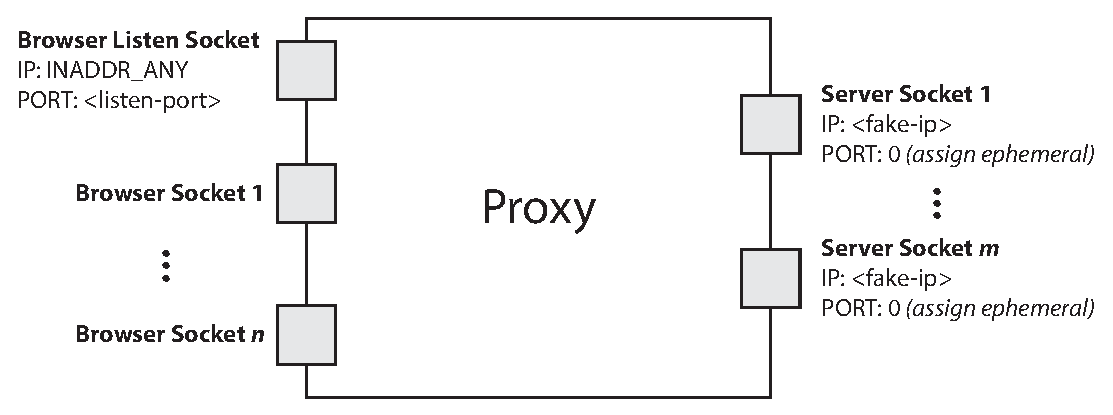
\includegraphics[width=0.6\textwidth]{figs/proxy.eps}
	\caption{Your proxy should listen for browser connections on
	\texttt{INADDR\_ANY} on the port specified on the command line. It should
	then connect to web servers on sockets that have been bound to the proxy's
	fake IP address (also specified on the command line).}

	\label{fig:proxy}
\end{figure}

Your proxy should accept multiple concurrent connections using
\texttt{select()}, as in project 1. It is fine to re-use \texttt{select()} and
HTTP parsing code from project 1.

\subsubsection{Throughput Calculation}
\label{sec:throughput-estimation}
Your proxy could estimate each stream's throughput once per chunk as
follows. Note the start time, $t_s$, of each chunk request (i.e., include
\texttt{time.h} and save a timestamp using \texttt{time()} when your proxy
receives a request from the player). Save another timestamp, $t_f$, when you
have finished receiving the chunk from the server.  Now, given the size of the
chunk, $B$, you can compute the throughput, $T$, your proxy saw for this
chunk:
\[
	T = \frac{B}{t_f - t_s}
\]


To smooth your throughput estimation, your proxy should use an
exponentially-weighted moving average (EWMA). Every time you make a new
measurement ($T_{new}$), update your current throughput estimate as follows:
\begin{equation}
	T_{current} = \alpha T_{new}  +  (1 - \alpha)T_{current}
\label{eq:ewma}
\end{equation}
The constant $0 \leq \alpha \leq 1$ controls the tradeoff between a smooth
throughput estimate ($\alpha$ closer to 0) and one that reacts quickly to
changes ($\alpha$ closer to 1). You will control $\alpha$ via a command line
argument. When a new stream starts, set $T_{current}$ to the lowest available
bitrate for that video.



\subsubsection{Choosing a Bitrate}

Once your proxy has calculated the connection's current throughput, it should
select the highest offered bitrate the connection can support. For this
project, we say a connection can support a bitrate if the average throughput is
at least 1.5 times the bitrate. For example, before your proxy should request
chunks encoded at 1000 Kbps, its current throughput estimate should be at least
1.5 Mbps.

Your proxy should learn which bitrates are available for a given video by
parsing the manifest file (the ``.f4m'' initially requested at the beginning of
the stream). The manifest is encoded in XML; each encoding of the video is
described by a \texttt{$<$media$>$} element, whose \texttt{bitrate} attribute
you should find.

Your proxy replaces each chunk request with a request for the same chunk at the
selected bitrate (in Kbps) by modifying the HTTP request's Request-URI. Video
chunk URIs are structured as follows:
\begin{center}
	\texttt{/path/to/video/$<$bitrate$>$Seq$<$num$>$-Frag$<$num$>$}
\end{center}

For example, suppose the player requests fragment 3 of chunk 2 of the video Big
Buck Bunny at 500 Kbps:
\begin{center}
	\texttt{/path/to/video/500Seg2-Frag3}
\end{center}
To switch to a higher bitrate, e.g., 1000 Kbps, the proxy should modify the URI
like this:
\begin{center}
	\texttt{/path/to/video/1000Seg2-Frag3}
\end{center}

\medskip \noindent \textbf{IMPORTANT:} When the video player requests
\texttt{big\_buck\_bunny.f4m}, you should instead return
\texttt{big\_buck\_bunny\_nolist.f4m}. This file does not list the available
bitrates, preventing the video player from attempting its own bitrate
adaptation. You proxy should, however, fetch \texttt{big\_buck\_bunny.f4m} for
itself (i.e., don't return it to the client) so you can parse the list of
available encodings as described above.


\subsubsection{Logging}
\label{sec:proxy-logging}

We require that your proxy create a log of its activity in a very particular
format. After each request, it should append the following line to the log:
\begin{center}
	\texttt{$<$time$>$ $<$duration$>$ $<$tput$>$ $<$avg-tput$>$ $<$bitrate$>$ $<$server-ip$>$ $<$chunkname$>$}
\end{center}

\begin{description}
	\item[\texttt{time}] The current time in seconds since the epoch.
	\item[\texttt{duration}] A floating point number representing the number of
	seconds it took to download this chunk from the server to the proxy.
	\item[\texttt{tput}] The throughput you measured for the current chunk in
	Kbps.
	\item[\texttt{avg-tput}] Your current EWMA throughput estimate in Kbps.
	\item[\texttt{bitrate}] The bitrate your proxy requested for this chunk in
	Kbps.
	\item[\texttt{server-ip}] The IP address of the server to which the proxy
	forwarded this request.
	\item[\texttt{chunkname}] The name of the file your proxy requested from
	the server (that is, the modified file name in the modified HTTP GET
	message).
\end{description}


\subsubsection{Running the Proxy}
\label{sec:running-proxy}

By running \texttt{make} in the root of your submission directory, we should be
able to create an executable called \texttt{proxy}, which should be invoked as
follows, \emph{even if not all arguments are functional at the first checkpoint}:
\begin{center}
	\texttt{./proxy $<$log$>$ $<$alpha$>$ $<$listen-port$>$ $<$fake-ip$>$ $<$dns-ip$>$ $<$dns-port$>$ [$<$www-ip$>$]}
\end{center}

\begin{description}
	\item[\texttt{log}] The file path to which you should log the messages
	described in \S\ref{sec:proxy-logging}.
	\item[\texttt{alpha}] A float in the range [0, 1]. Uses this as the
	coefficient in your EWMA throughput estimate (Equation~\ref{eq:ewma}).
	\item[\texttt{listen-port}] The TCP port your proxy should listen on for
	accepting connections from your browser.
	\item[\texttt{fake-ip}] Your proxy should bind to this IP address \emph{for
	outbound connections to the web servers}. You should \emph{not} bind your
	browser listen socket to this IP address --- bind that socket to
	\texttt{INADDR\_ANY}.
	\item[\texttt{dns-ip}] IP address of the DNS server.
	\item[\texttt{dns-port}] UDP port DNS server listens on.
	\item[\texttt{www-ip}] Your proxy should accept an optional argument
	specifying the IP address of the web server from which it should request
	video chunks. If this argument is not present, your proxy should obtain the
	web server's IP address by querying your DNS server for the name \theurl.
\end{description}

To play a video through your proxy, point a browser on your VM to the URL\\
\texttt{http://localhost:$<$listen-port$>$/index.html}. (You can also configure
VirtualBox's port forwarding to send traffic from \texttt{$<$listen-port$>$} on
the host machine to \texttt{$<$listen-port$>$} on your VM; this way you can
play the video from your own web browser.)





\section{DNS Load Balancing}
\label{sec:dns}

To spread the load of serving videos among a group of servers, most CDNs
perform some kind of load balancing. A common technique is to configure the
CDN's authoritative DNS server to resolve a single domain name to one out of a
set of IP addresses belonging to replicated content servers. The DNS server can
use various strategies to spread the load, e.g., round-robin, shortest
geographic distance, or current server load (which requires servers to
periodically report their statuses to the DNS server).

\subsection{Requirements}

You will write a simple DNS server that implements load balancing two different
ways: round-robin and geographic distance.

\bigskip \noindent \textbf{Checkpoint 2:}~~~DNS load balancing comes into play
at the second checkpoint. You must implement the two load balancing strategies
described below. In order for you proxy to be able to query your DNS server,
you must also write an accompanying DNS resolution library (see
\S\ref{sec:dns-details} for details).

\medskip \noindent \textit{(1) Round robin.} First, implement a simple
round-robin based DNS load balancer. Your DNS process should take as input a
list of video server IP addresses (the topology's \texttt{.servers} file ---
\S\ref{sec:starter-files}) on the command line (\S\ref{sec:dns-details}); it
responds to each request to resolve the name \theurl by returning the next IP
address in the list, cycling back to the beginning when the list is exhausted.

\medskip \noindent \textit{(2) Geographic distance.} Next you'll make your DNS
server somewhat more sophisticated --- must return the closest video server to
the client based on the client's IP address. In the real world, this would be
done by querying a database mapping IP prefixes to geographic locations. In
your implementation, you will pretend that a link state routing protocol (e.g.,
OSPF) is used Internet-wide and that your DNS server participates in it. Your
DNS server must process link state advertisements (LSAs), build a graph of the
entire network, and run Dijkstra's shortest path algorithm on the graph to
determine the closest video server for a given client.

\emph{You do not need to implement LSA flooding.} We will provide you with a
file containing a list of LSAs which your server would have received had you
actually implemented LSA flooding.  The file contains one LSA per line,
formatted as follows:
\begin{center}
	\texttt{$<$sender$>$ $<$sequence number$>$ $<$neighbors$>$}
\end{center}

\begin{description}
	\item[\texttt{sender}] The IP address of the node that originated this LSA. 
	\item[\texttt{sequence number}] An integer allowing you to order the LSAs
	from a given sender. Each node sends multiple LSAs; you should accept only
	the most recent (\emph{even if they arrive out of order}).  You may assume
	sequence numbers don't wrap back to zero within the LSA file and that nodes
	in the network never reboot and start over at zero.
	\item[\texttt{neighbors}] A comma-separated string of IP addresses denoting
	the sender's immediate (directly connected) neighbors. 
\end{description}



\subsection{Implementation Details}
\label{sec:dns-details}

Your DNS implementation will consist of two pieces: your DNS server and your
client-side resolution library. The two pieces should communicate using the DNS
message formats defined in section 4.1 of RFC 1035. To make your life easier:

\begin{description}
	\item[\texttt{AA}] Set this to 0 in requests, 1 in responses.
	\item[\texttt{RD}] Set this to 0 in all messages.
	\item[\texttt{RA}] Set this to 0 in all messages.
	\item[\texttt{Z}] Set this to 0 in all messages.
	\item[\texttt{NSCOUNT}] Set this to 0 in all messages.
	\item[\texttt{ARCOUNT}] Set this to 0 in all messages.
	\item[\texttt{QTYPE}] Set this to 1 in all requests (asking for an A record).
	\item[\texttt{QCLASS}] Set this to 1 in all requests (asking for an IP address).
	\item[\texttt{TYPE}] Set this to 1 in all responses (returning an A record).
	\item[\texttt{CLASS}] Set this to 1 in all responses (returning an IP address).
	\item[\texttt{TTL}] Set this to 0 in all responses (no caching).
\end{description}


\subsubsection{DNS Server}
\label{sec:dns-server-details}

Your DNS server will operate over UDP. It will bind to an IP address and port
specified as command line arguments. It need only respond to requests for
\theurl; any other requests should generate a response with \texttt{RCODE} 3.
By running \texttt{make} in the root of your submission directory, we should be
able to create an executable called \texttt{nameserver}, which should be
invoked as follows \emph{even if not all arguments are functional}:
\begin{center}
	\texttt{./nameserver [-r] $<$log$>$ $<$ip$>$ $<$port$>$ $<$servers$>$ $<$LSAs$>$}
\end{center}

\begin{description}
	\item[\texttt{-r}] If present, this flag indicates the server should
	perform round-robin load balancing instead of processing LSAs and returing
	the client's closest server.
	\item[\texttt{log}] The file path to which you should log the messages
	as described below.
	\item[\texttt{ip}] The IP address on which your server should listen.
	\item[\texttt{port}] The UDP port on which your server should listen.
	\item[\texttt{servers}] A text file containing a list of IP addresses, one
	per line, belonging to content servers.
	\item[\texttt{LSAs}] A text file containing a list of LSAs, one per line,
	in the format described above.
\end{description}

\bigskip \noindent \textbf{Logging}~~Like your proxy, your DNS server must log
its activity in a specific format.  For each valid DNS query it services, it
should append the following line to the log:
\begin{center}
	\texttt{$<$time$>$ $<$client-ip$>$ $<$query-name$>$ $<$response-ip$>$}
\end{center}

\begin{description}
	\item[\texttt{time}] The current time in seconds since the epoch.
	\item[\texttt{client-ip}] The IP address of the client who sent the query.
	\item[\texttt{query-name}] The hostname the client is trying to resolve.
	\item[\texttt{response-ip}] The IP address you return in response.
\end{description}



\subsubsection{Resolution Library}
The library offers one function: \texttt{resolve()}. We have provided the
interface in \texttt{mydns.h}; you are to write the accompanying implementation
in a file named \texttt{mydns.c}. Your proxy will use your resolver by
including \texttt{mydns.h} and calling \texttt{resolve()} at the beginning of
each new connection.




\section{Development Environment}
\label{sec:starter}

For this project, we are providing a virtual machine pre-configured with the
software you will need. We strongly recommend that you do all development and
testing in this VM; your code must compile and run correctly on this image as
we will be using it for grading. This section describes the VM and the starter
code it contains.

\subsection{Virtual Box}

The virtual machine disk (VMDK) we provide was created using VirtualBox, though
you may be able to use it with other virtualization software. VirtualBox is a
free download for Windows, OSX, and Linux on \url{https://www.virtualbox.org}.
We've already set up an admin account:
\begin{description}
	\item[Username:] proj3
	\item[Password:] proj3
\end{description}


\subsection{Starter Files}
\label{sec:starter-files}

You will find the following files in
\texttt{/home/proj3/bitrate-project-starter}. This directory is a git
repository; as we find bugs in the starter code and commit fixes, you can get
the update versions with a \texttt{git pull}.
\begin{description}
	\item[\texttt{mydns.h}] The interface for your DNS resolution library (\S\ref{sec:dns-details}).

	\item[\texttt{common}] Common code used by our network simulation and LSA generation scripts.

	\item[\texttt{lsa}]
	\item[\texttt{lsa/genlsa.py}] Generates LSAs for a provided network
	topology. You may use this to generate LSA files beyond those we provide,
	if you like.

	\item[\texttt{netsim}]
	\item[\texttt{netsim/netsim.py}] This script controls the simulated
	network; see \S\ref{sec:netsim}.
	\item[\texttt{netsim/tc\_setup.py}] This script adjusts link
	characteristics (BW and latency) in the simulated network. It is called by
	\texttt{netsim.py}; you do not need to interact with it directly.
	\item[\texttt{netsim/apache\_setup.py}] This file contains code used by
	\texttt{netsim.py} to start and stop Apache instances on the IP addresses
	in your \texttt{.servers} file; you do not need to interact with it
	directly.

	\item[\texttt{grapher.py}] A script to produce plots of link utilization, fairness, and smoothness from log files. (See \S\ref{sec:proxy-reqs}.)

	\item[\texttt{topos}]
	\item[\texttt{topos/topo1}]
	\item[\texttt{topos/topo1/topo1.clients}] A list of IP addresses, one per line, for the proxies. (Used by \texttt{netsim.py} to create a fake network interface for each proxy.)
	\item[\texttt{topos/topo1/topo1.servers}] A list of IP addresses, one per line, for the video servers. (Used by your DNS server and by \texttt{netsim.py} to create a fake interface for each server.)
	\item[\texttt{topos/topo1/topo1.dns}] A single IP address for your DNS server. (Used by \texttt{netsim.py} to create a fake interface for your DNS server.)
	\item[\texttt{topos/topo1/topo1.links}] A list of links in the simulated network. (Used by \texttt{genlsa.py}.)
	\item[\texttt{topos/topo1/topo1.bottlenecks}] A list of bottleneck links to be used in \texttt{topo1.events}. (See \S\ref{sec:netsim}.)
	\item[\texttt{topos/topo1/topo1.events}] A list of changes in link characteristics (BW and latency) to ``play.'' See the comments in the file. (Used by \texttt{netsim.py}.)
	\item[\texttt{topos/topo1/topo1.lsa}] A list of LSAs heard by the DNS server in this topology.
	\item[\texttt{topos/topo1/topo1.pdf}] A picture of the network.
	\item[\texttt{topos/topo2}]
	\item[\texttt{...}]

\end{description}


\subsection{Network Simulation}
\label{sec:netsim}

To test your system, you will run everything (proxies, servers, and DNS server)
on a simulated network in the VM. You control the simulated network with the
\texttt{netsim.py} script. You need to provide the script with a directory
containing a network topology, which consists of several files. We provide two
sample toplogies; feel free to create your own. See \S\ref{sec:starter-files}
for a description of each of the files comprising a topology. Note that
\texttt{netsim.py} requires that each constituent file's prefix match the name
of the topology (e.g., in the \texttt{topo1} directory, files are named
\texttt{topo1.clients}, \texttt{topo1.servers}, etc.).

To start the network from the \texttt{netsim} directory:
\begin{center}
	\texttt{./netsim.py $<$topology$>$ start}
\end{center}
Starting the network creates a fake network interface for each IP address in
the \texttt{.clients}, \texttt{.servers}, and \texttt{.dns} files; this allows
your proxies, Apache instances, and DNS server to bind to these IP addresses.

To stop it once started (thereby removing the fake interfaces), run:
\begin{center}
	\texttt{./netsim.py $<$topology$>$ stop}
\end{center}

To facilitate testing your adaptive bitrate selection, the simulator can vary
the bandwidth and latency of any link designated as a bottleneck in your
topology's \texttt{.bottlenecks} file. (Bottleneck links must be declared
because our simulator limits you to adjusting the characteristics of only one
link between any pair of endpoints. This also means that some topologies simply
cannot be simulated by our simulator.) To do so, add link changes to the
\texttt{.events} file you pass to \texttt{netsim.py}. Events can run
automatically according to timings specified in the file or they can wait to
run until triggered by the user (see \texttt{topos/topo1/topo1.events} for an
example). When your \texttt{.events} file is ready, tell \texttt{netsim.py} to
run it:
\begin{center}
	\texttt{./netsim.py $<$topology$>$ run}
\end{center}
Note that you must start the network before running any events. You can issue
the \texttt{run} commands as many times as you want without restarting the
network. You may modify the \texttt{.events} file between runs, but you must
\emph{not} modify any other topology files, including the \texttt{.bottlenecks}
file, without restarting the network. Also note that the links stay as the last
event configured them even when \texttt{netsim.py} finishes running.

\medskip \noindent \textbf{Link State Advertisements}~~You'll notice that the
simulated network described above doesn't actually contain any routers ---
we've taken them out of the picture to make your lives simpler by allowing you
to independently set the bandwidth between any pair of endpoints (fake NICs).
But, for the sake of the LSAs your DNS server needs to process, we need to
\emph{pretend that there are fake routers}. Yes, this is a tad confusing and
contrived. Sorry. Deal with it. So, in each sample topology, we provide a
\texttt{.links} file containing pairs of network elements (hosts or routers)
between which there is a link in this pretend fake network. If the endpoint is
a host, use its fake IP address in the \texttt{.links} file. If it is a pretend
fake router, we use any string (e.g., ``router1'').

If want to make a new LSA file based on a new network topology for your
testing, you can generate one using the \texttt{genlsa.py} script (run
\texttt{./genlsa.py -h} for information on how to use it).





%\subsection{Videos}
%\label{sec:videos}
%
%\textbf{TODO: describe video chunks/manifest}



\subsection{Apache}
\label{sec:apache}

You will use the Apache web server to server the video files.
\texttt{netsim.py} automatically starts an instance of Apache for you on each
IP address listed in your topology's \texttt{.servers} file. Each instance
listens on port 8080 and is configured to serve files from \texttt{/var/www};
we have put sample video chunks here for you.




\section{Hand In}

\subsection{What to Submit}

You will submit your code as a tarball named \texttt{team$<$num$>$.tar}.
Untarring this file should give us a directory named \texttt{handin} which
should contain the following:

\medskip \noindent \textbf{Checkpoint 1:}
\begin{itemize}
	\item \texttt{Makefile} --- Running \texttt{make} should produce an
	executable named \texttt{proxy}, as described in \S\ref{sec:running-proxy}.

	\item \texttt{writeup.pdf} --- This should contain the plots and analysis
	described in \S\ref{sec:proxy-reqs}. 

	\item \texttt{src} --- A directory named \texttt{src} containing your
	source code. You may organize your code within this directory as you see
	fit.
\end{itemize}


\medskip \noindent \textbf{Checkpoint 2 (Final Submission):}
\begin{itemize}
	\item \texttt{Makefile} --- Running \texttt{make} should produce an
	executable named \texttt{proxy}, as described in \S\ref{sec:running-proxy},
	and an executable named \texttt{nameserver}, as described in
	\S\ref{sec:dns-server-details}.

	\item \texttt{writeup.pdf} --- This should contain the plots and analysis
	described in \S\ref{sec:proxy-reqs}. 

	\item \texttt{src} --- A directory named \texttt{src} containing your
	source code. You may organize your code within this directory as you see
	fit, with the exception that we should find \texttt{mydns.c} immediately
	inside \texttt{src}.
\end{itemize}


\subsection{Where to Submit}

You will submit your code using Autolab (\url{https://autolab.cs.cmu.edu}). If
you can't log in, let us know ASAP. 

When you first log in, you'll be asked to choose a nickname. This nickname will
be displayed along with you score on a scoreboard visible to the entire class,
so don't use your real name if you'd like to keep your score private. Once you
log in, choose ``Check partner'' and verify that your partner is correct; if
not, let us know ASAP.

To submit your code, choose ``15-441: Computer Networks (f13)'' $>$
``project3cp1'' and then upload your tarball. Only one team member needs to
upload code. You may upload your code as many times as you like until the
deadline. The grader typically takes 2-3 minutes but make take longer depending
on system load.

Since we will not be using git for submission, you are not required to use it.
However, we \emph{strongly} recommend using a git repository for development,
especially since you are writing code with a partner.


\section{Grading}

Your grade will consist of the following components:

\smallskip \noindent \textbf{Checkpoint 1} \textit{(10 points)}
\begin{itemize}
	\item Proxy
	\item Writeup (completion points)
\end{itemize}

\smallskip \noindent \textbf{DNS} \textit{(35 points)}
\begin{itemize}
	\item DNS client-side resolution library
	\item Correct DNS message format
	\item Round robin load balancing
	\item LSA processing and ``geographic'' load balancing
\end{itemize}

\smallskip \noindent \textbf{Proxy} \textit{(35 points)}
\begin{itemize}
	\item Throughput estimation (EWMA)
	\item Adaptive bitrate selection
\end{itemize}

\smallskip \noindent \textbf{Writeup} \textit{(15 points)}
\begin{itemize}
	\item Plots of utilization, fairness, and smoothness for $\alpha \in \{0.1, 0.5, 0.9\}$
	\item Discussion of tradeoffs for varying $\alpha$
\end{itemize}

\smallskip \noindent \textbf{Style} \textit{(5 points)}
\begin{itemize}
	\item Code thoroughly commented
	\item Code organized and modular
	\item README listing your files and what they contain
\end{itemize}



\end{document}
